\chapter{Peer-to-peer file distribution}
\label{cha:distribution}
This chapter discusses the design of the file distribution mechanism in NanoTorrent. These mechanisms enable peers to connect with each other, exchange download progress information and request file data.

Section \ref{sec:distrib:requirements} lists the requirements for the distribution. Section \ref{sec:distrib:piece} explains the use of fixed-size pieces to subdivide the distributed file. The management of peer connections is discussed in \ref{sec:distrib:connection}, and the actual piece exchange is described in \ref{sec:distrib:exchange}. The local peer discovery mechanism described in \ref{sec:discovery:local} allows for an optimization in the piece exchange, which is discussed in \ref{sec:distrib:multicast}. Section \ref{sec:distrib:conclusion} rounds up the chapter with a conclusion.

\section{Requirements}
\label{sec:distrib:requirements}
The distributed file must fit in the non-volatile storage of every targeted node, and thus its size is limited. Whereas files distributed on the Internet can be several \glspl{GB} in size, \gls{WSN} nodes can only store files in the orders of a couple of \glspl{KB}. For example, the \gls{EEPROM} of the AVR Zigduino r2 platform, (used in the evaluation in chapter \ref{cha:evaluation}) can hold up to 4 KB of data \cite{zigduino-manual}. The file distribution protocol is dimensioned to work well with these relatively small files, in its current form up to 64 \gls{KB} ($2^{16}$ bytes).

The protocol should attempt to prevent redundant communications. For examples, peers should not request parts of the files from another peer if they do not know whether the other peer already has that part available. Therefore, peers should advertise information about their own download progress to others so they can make informed requests. This implies that peers need to retain stateful information about other peers.

Peers should try to balance the overall load on the \gls{P2P} network. If a certain piece of the file were only available at one single peer (which is often the case with an \gls{initial-seed} early on in the \gls{swarm}'s lifetime), that peer could become overloaded when other peers do not properly coordinate their requests. In the worst case, a failure of that single peer could prevent the rest of the network from receiving the whole file. The protocol should try to relieve peers with highly wanted file pieces, and prioritize their distribution over more commonly available pieces.

File distribution must be robust against corruptions and transmission errors. For example, when distributing a new program binary, it is crucial for the program's correctness and stability that the received file is bit-for-bit identical to the original. Therefore, \glspl{peer} must be able to independently verify the integrity of the received file in its entirety.

\section{Pieces}
\label{sec:distrib:piece}
NanoTorrent uses the same approach as BitTorrent to subdivide the distributed file in fixed-size \emph{pieces} which can be independently distributed over the \gls{P2P} network. This allows peers to retrieve them in any order and download multiple pieces from multiple peers in parallel (see \ref{sec:related:bittorrent}).

All information about a torrent's pieces are contained in the \emph{\gls{torrent-info}}, which is part of the \gls{torrent-desc} (detailed in \ref{sec:discovery:torrent-desc}). Peers can verify the integrity of the entire file by verifying the integrity of each individual piece. The SHA-1 hash of the torrent information (further abbreviated to \emph{info hash}) is used to tag all messages exchanged between peers, to ensure that messages for different torrents do not interfere with each other.

\section{Peer connections}
\label{sec:distrib:connection}
Peers can discover other peers in two ways: they can find out about another peer through the tracker (detailed in \ref{sec:discovery:tracker}), or they receive a message from another peer (which includes local peer discovery  from \ref{sec:discovery:local}). Both give the peer an \gls{IPv6} address of another peer, which they can use to directly communicate with the peer.

However, peers need to maintain some connection state for each peer they are communicating with:
\begin{itemize}
\item The peer's \gls{IPv6} address, for sending messages. This also acts as a `key' for the connection's state, allowing the peer to find the correct connection state when receiving messages from the peer.
\item The set of pieces available at that peer. This allows the local peer to find out which missing pieces are available at which connected peers, so it can send piece requests to the right peer.
\item The time of the last message received from that peer. This acts as a heartbeat, so the local peer can clean up this connection state if the other peer stops sending periodic messages.
\item Information about the current pending piece request to that peer. This allows the peer to track which pieces it is expecting to receive from which peers, and what parts of the pending pieces it has already received (see \ref{sec:distrib:exchange}).
\end{itemize}

The protocol specifies two types of messages to manage peer connections: \texttt{have} and \texttt{close} messages. A \texttt{have} message informs others of a peer's set of currently available pieces. Peers send this message periodically to keep their heartbeat alive at other peers, and when they have made new progress on their own download and want to notify others. A \texttt{close} message informs another peer that it should close the connection with the sending peer and clean up its connection state. This message is sent when a peer decides to close one of its opened connections.

To set up a connection, a peer simply allocates some connection state locally and can then start sending messages to the other peer. Depending on how the other peer was discovered, the first message sent could be a periodic \texttt{have} message (when the peer doesn't know anything yet about the available pieces), or an immediate piece data request (when the peer already knows about some of the available pieces).

To maintain its peer connections, a peer must periodically send a heartbeat to inform them about its own set of available pieces (using a \texttt{have} message). This lets other peers that this peer is still alive (and its heartbeat timer should be refreshed) and updates them on the current set of available pieces. If the other peer does not yet have a connection state for this peer, it can decide to set one up so it can send requests to this peer.

Keeping the view on the available pieces at other peers up-to-date is critical to achieve a fast file distribution to all peers. Therefore, this information is also piggy-backed onto every exchanged peer message. Peers could also decide to send their next \emph{have} heartbeat immediately after completing the download of a piece. However, this has the risk of flooding the network when many pieces are completed at around the same time. As a compromise, the next heartbeat only gets re-scheduled to a slightly earlier time whenever a piece is completed.

Since peers need resources to allocate and maintain their peer connections, the amount of simultaneously open peer connections is limited. This also means that when one peer creates a connection to another peer, the other peer doesn't necessarily have to do the same. In that case, the other peer \emph{immediately} sends a \texttt{close} message to indicate that it won't be able to maintain its side of the connection and the original peer should clean up its connection state. After cleaning up the failed connection, the peer can continue to try connecting with a different peer instead.

One exception to these fast \texttt{close} semantics shows up when taking into account the multicast \texttt{have} messages used in local peer discovery (see \ref{sec:discovery:local}). Whereas regular \texttt{have} messages are sent to initiate a connection to a \emph{known} peer, these multicast messages are sent to discover one or more \emph{unknown} neighbouring peers. If every peer receiving a multicast advertisement would reply with a useless \texttt{close} message, the protocol's performance would degrade drastically. To prevent this, peers only send a \texttt{close} reply when the received \texttt{have} message is directed to only them (i.e. when the message is destined to a \emph{unicast} address as opposed to a multicast address).

\section{Piece exchange}
\label{sec:distrib:exchange}
The protocol provides request-reply style messages to exchange piece data with \texttt{data request} and \texttt{data reply} messages. A \texttt{data request} includes the index of the requested piece (following the order in the \gls{torrent-info}) and the offset of the first data byte in the response. A \texttt{data reply} contains the same fields, followed by the actual data bytes. Peers can freely choose how many bytes they send in a \texttt{data reply} depending on their own capabilities, although they should try to fill the whole packet with piece data to reduce the total number of requests needed to exchange the whole piece.

A peer starts by selecting a piece to request. They can use any piece selection strategy, however the current implementation uses the same \emph{rarest-first} policy as BitTorrent. This policy selects the piece which is the \emph{least common} of all pieces available at all currently connected peers, in an attempt to help make these `rare' pieces more common in the network and balance the overall load.

Following, the peer sends the first \texttt{data request} with byte offset \texttt{0} to request the first part of the piece. After receiving a corresponding \texttt{data reply}, the peer writes the received data to storage, increments the byte offset with the size of the response data and sends the next \texttt{data request}.

When all data of a piece is received, the peer calculates the SHA-1 hash of the downloaded data and compares it to the expected piece hash from the \gls{torrent-info}. Only if these match, should the peer accept the piece and notify others about the newly available piece. If there is a mismatch, the peer assumes that the data was corrupted and retries the piece exchange from scratch. By doing this for every piece, a peer can verify the integrity of the \emph{entire file} and be confident that it has indeed received a bit-for-bit exact copy of the file.

\section{Multicast piece delivery}
\label{sec:distrib:multicast}
With local peer discovery (explained in \ref{sec:discovery:local}), NanoTorrent can already find direct neighbours which are also downloading the same torrent. To fully take advantage of this locality however, peers should also try to efficiently exchange pieces with their immediate neighbours.

This is done by sending \texttt{data reply} messages directed to a local peer (identified by a link-local \gls{IPv6} address) to \emph{all} local peers as a link-local multicast, rather than a regular link-local unicast. This allows a single peer to distribute a piece to all of its neighbours at once, rather than sending many individual \texttt{data reply} messages.

Of course, this means that a peer must be able to handle incoming \texttt{data reply} messages for which it is \emph{not} the original requester. If a peer receives data from the start of a piece (byte offset \texttt{0}) and it does not yet have a pending request for the sending peer, it can create a new request on the fly and process the incoming data as part of this request. Subsequently received data with other byte offsets can then be handled as part of this newly created request. If the peer already has a different pending request, it cannot create a second request and will have to request it later on. This could be improved to allow multiple pending requests, at the cost of more complex request tracking logic.

Figure \ref{fig:distribution:multicast} shows an example interaction between three local peers. The first peer has a connection with the second peer, and sends a \texttt{data request} for one of the available pieces. The second peer sends the \texttt{data reply} as a multicast message to all direct neighbours. The third peer manages to pick up this message from a previously unknown local peer, adds it to its peer connections, creates a pending piece request on-the-fly and stores the received data as part of that request. It then sends a unicast \texttt{data request} for the next part of the piece from the second peer. The second peer now discovers this new third peer and again sends a \texttt{data reply} to all neighbours. This shows how multiple neighbours can receive data from a single multicast piece exchange, and how such an exchange can also allow two peers to discover each other without a single \texttt{have} announcement.

\begin{figure}
    \centering
    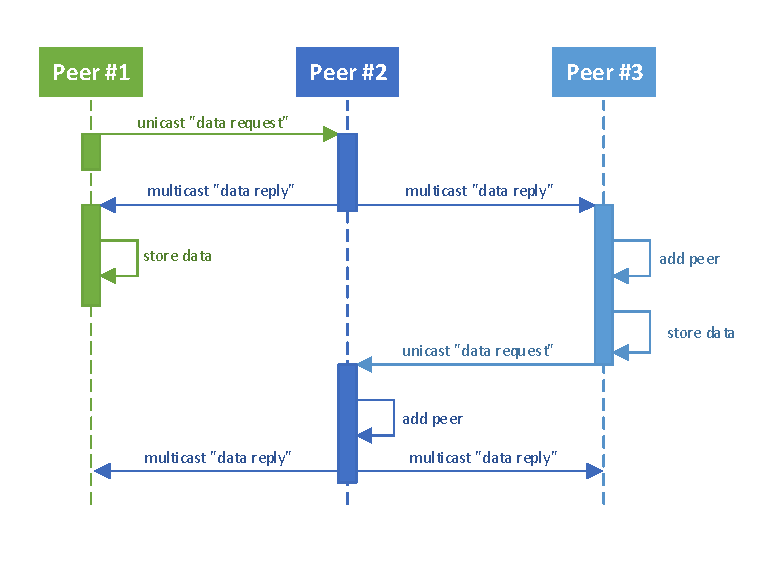
\includegraphics[width=\textwidth]{diagrams/piece-exchange.pdf}
    \caption[Sequence diagram of multicast piece delivery]{Sequence diagram of multicast piece delivery. The multicast \texttt{data reply} allows multiple peers to receive piece data, and also act as implicit local peer discovery announcements.}
    \label{fig:distribution:multicast}
\end{figure}

\section{Conclusion}
\label{sec:distrib:conclusion}
The file is subdivided into fixed-size pieces, which can be distributed over the \gls{P2P} network independently. All information about these pieces is contained in the \gls{torrent-desc}, which must be delivered to every node in some way before starting the torrent download. The SHA-1 hashes of every piece allow a peer to verify the integrity of every piece and, by extension, the entire file.

Peers try to connect with their discovered peer in order to exchange pieces. They maintain some state about what pieces are available at the other end, and which pieces are currently being requested by connected peers. Peers periodically send \texttt{have} messages to keep other peers informed about their download progress, and to indicate that they are still alive.

Pieces are exchanged using a simply request-reply protocol, where one peer sends requests for a part of a piece and the other peer replies with the corresponding data. After all the data of a piece is received, the peer compares the calculated SHA-1 hash with the expected hash from the \gls{torrent-desc}. When the verification succeeds, the peer can request its next missing piece and start serving requests for the received piece itself.

To exploit the locality of peers discovered through local peer discovery, peers send their data replies destined to a local peer to \emph{all} local peers using a link-local multicast. Receiving peers attempt to piggy-back onto this piece exchange, allowing a single piece request to serve many local peers. This enables a faster and more efficient distribution inside clusters of nodes.
